\documentclass[aspectratio=169,11pt]{beamer}
\usepackage[utf8]{inputenc}
\usepackage[T1]{fontenc}
\usepackage{lmodern}
\usepackage{amsmath}
\usepackage{amsfonts}
\usepackage{amssymb}
\usepackage{graphicx}
\usetheme{default}
\usepackage{epstopdf}
\usepackage{subfigure}
\usepackage{tabularx}
\usepackage{booktabs}

\title{Community Detection With Katz and Eigenvector Centrality}
\subtitle{Complex Networks 2019}
\author{Mark Ditsworth\thanks{markditsworth@protonmail.com}, Justin Ruths\thanks{jruths@utdallas.edu}}
\institute{University of Texas at Dallas}
\date{December 10, 2019}
\begin{document}
\begin{frame}[plain]
    \maketitle
    
\end{frame}

\begin{frame}{Community Detection}
	\textbf{Goal:} Given a network, determine which nodes belong to groups based on their network activity\\
	\vspace{15pt}
	\textbf{Two Primary Approaches:}\\
	\textit{Louvain} -- Iteratively check permutations of community assignments using a modularity maximization heuristic\cite{louvain}\\
	\textit{Spectral} -- Find the leading eigenvector of the modularity matrix and transform to discrete community identifiers\cite{spectral}\\
	\vspace{15pt}
	Both approaches can be time and/or resource consuming for large networks.\\
	\vspace{15pt}
	\textbf{We show another method based on comparing Katz centrality and Eigenvector centrality that is more scalable on large networks.}
\end{frame}

\begin{frame}{Localization of Eigenvector Centrality in Modular Networks}
	\begin{tabular}{cc}
		\begin{tabular}{l}
			Eigenvector centrality ($\mathbf{x}$) \\ calculated by leading eigenvector of\\ adjacency matrix ($\mathbf{A}$)\cite{evc}\\\\
			\( \mathbf{x} = \frac{1}{\lambda_1}\mathbf{A}\mathbf{x}\)\\\\
				Reduced information leads to \\
				"localization" of centrality.
		\end{tabular}
		& \begin{tabular}{c}
			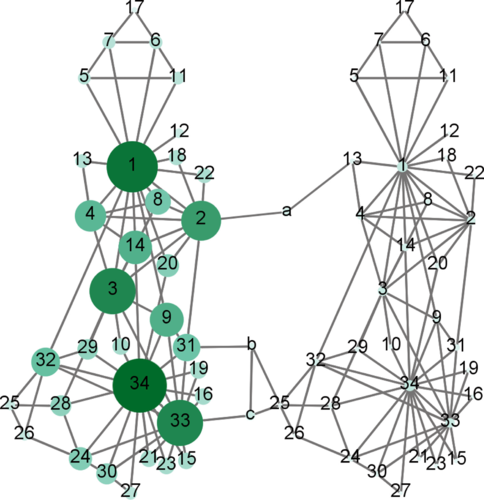
\includegraphics[scale=0.3]{modular_example.png}\\
			Double-karate network with 3-node cut set.\\
			Node size and darkness increase\\with eigenvector centrality\cite{localization}
		\end{tabular}
	\end{tabular}
\end{frame}

\begin{frame}{Robust Katz Centrality Complements Eigenvector Centrality}
			The following, illustrated in \cite{localization}, shows that Katz Centrality spans the entire eigenbasis of the adjacency matrix $\mathbf{A}$ of an undirected network.
			\\
			Katz Centrality\cite{katz} is given by,\\
			\begin{equation*}
			\mathbf{x} = (I-\alpha \mathbf{A})^{-1}~\beta\textbf{1}~,~\alpha < \frac{1}{\lambda_1}
			\end{equation*}\\
			The inverse operation can be expressed as a power series,
			\begin{equation*}
			(I - \alpha \mathbf{A})^{-1} = I + \alpha \mathbf{A} + \alpha^2 \mathbf{A}^2 + \alpha^3 \mathbf{A}^3 + \dotsi~
			\end{equation*}\\
			The vector $\beta\textbf{1}$ can be expressed as a linear combination of the orthogonal eignvectors of $\mathbf{A}$: $\mathbf{u}_1 \dots \mathbf{u}_n$\\
			\begin{equation*}
			 \mathbf{x} = (I + \alpha \mathbf{A} + \alpha^2 \mathbf{A}^2 + \dotsi ) (a_1\mathbf{u}_1 + a_2\mathbf{u_2} + \dotsi + a_n\mathbf{u}_n)
			\end{equation*}\\
			Thus, $ \mathbf{x} = a_1\mathbf{u}_1\sum_{k=0}^{\infty}(\alpha\lambda_1)^k +
			\dotsi +
			a_n\mathbf{u}_n\sum_{k=0}^{\infty}(\alpha\lambda_n)^k$
\end{frame}

\begin{frame}{Katz-Eigenvector Centrality Plot Identifies Modular Communities}
	
	\begin{figure}
		\centering
		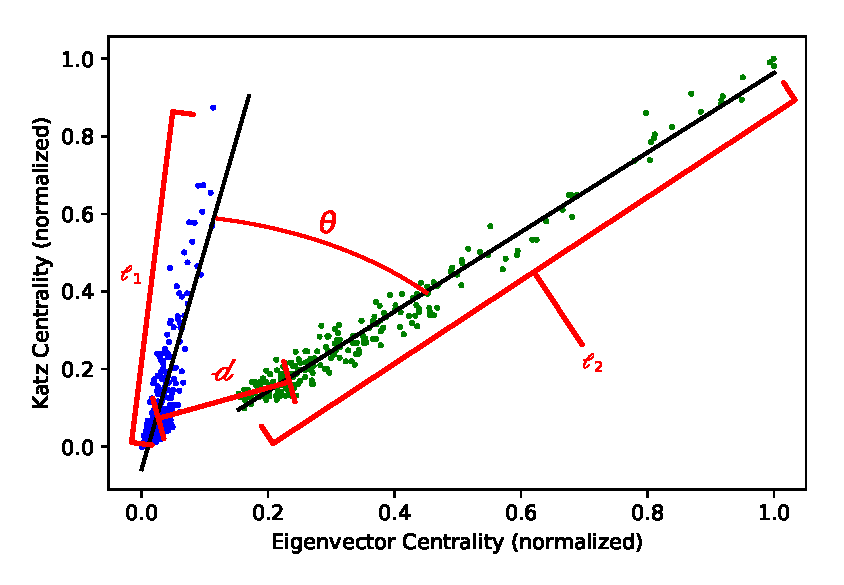
\includegraphics[scale=0.6]{./example_ba}
		\caption{Ad-hoc modular network with two Barabasi-Albert\cite{BA} random networks (n=250) joined by 800 randomly placed edges.}
	\end{figure}
\end{frame}

\begin{frame}{Modularity, Density Affect The KE Plot Clusters' Angle}
	\begin{figure}
		\centering
		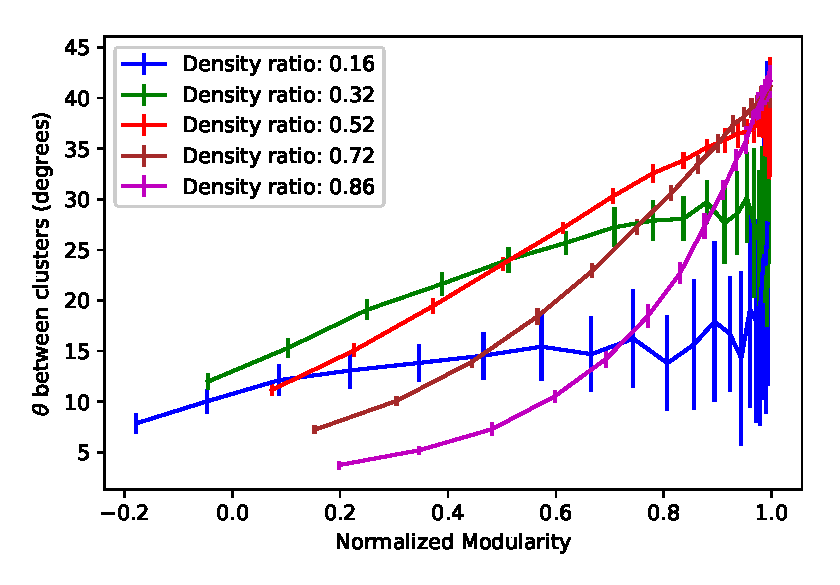
\includegraphics[scale=0.7]{theta_ba.eps}
	\end{figure}
\end{frame}

\begin{frame}{Modularity, Density Affect The KE Plot Clusters' Distance}
	\begin{figure}
		\centering
		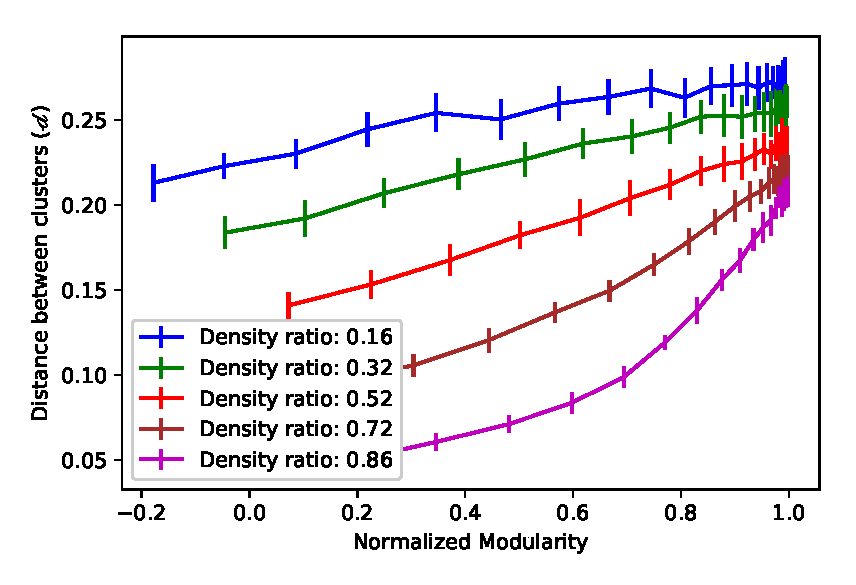
\includegraphics[scale=0.7]{distance_ba.eps}
	\end{figure}
\end{frame}

\begin{frame}{Modularity, Density Affect The KE Plot Clusters' Length Ratio}
	\begin{figure}
		\centering
		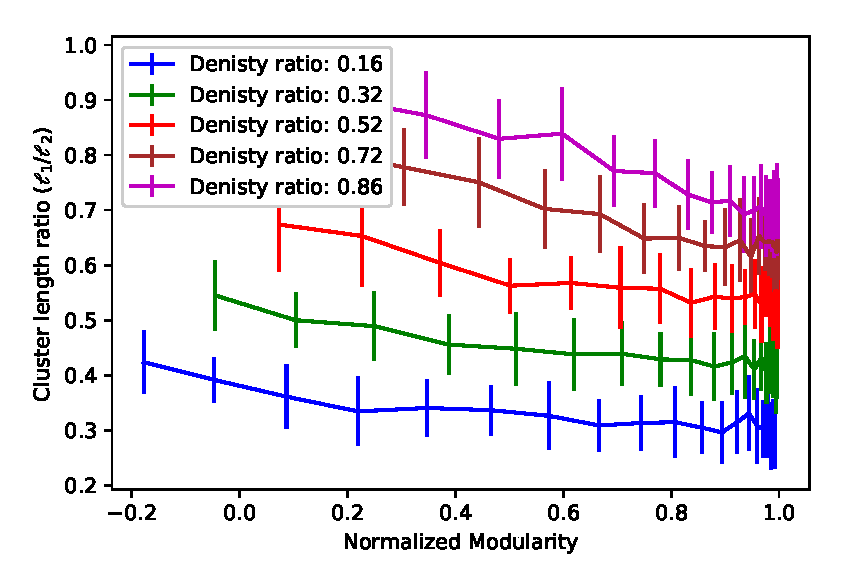
\includegraphics[scale=0.7]{length_ba.eps}
	\end{figure}
\end{frame}


\begin{frame}{KE Plot Identifies Communities in Real-World Networks}
	\begin{figure}
		\centering
		\subfigure[DBLP network\cite{dblp}]{
			\label{fig:dblp_cluster}
			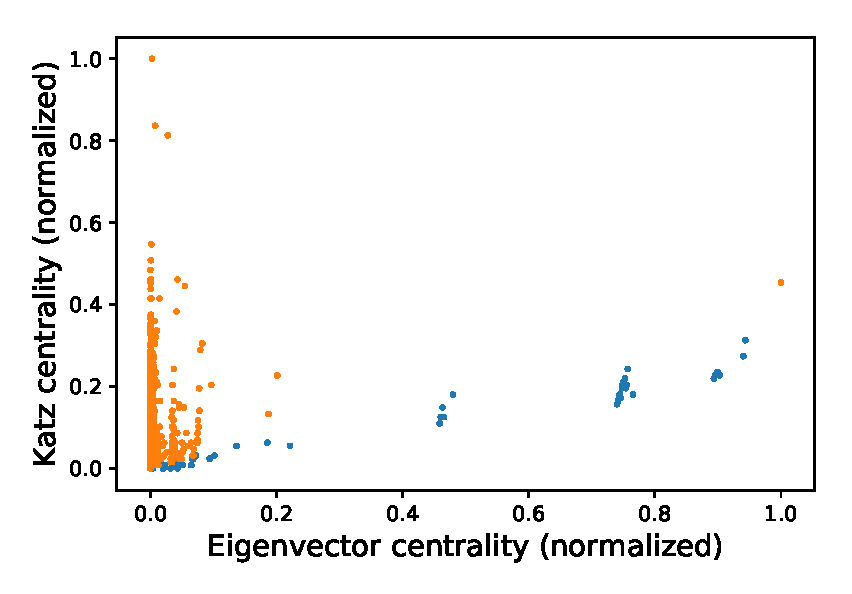
\includegraphics[width=0.45\linewidth]{dblp_ke.eps}}
		\subfigure[Amazon product network\cite{amazon}]{
			\label{fig:amazon_product}
			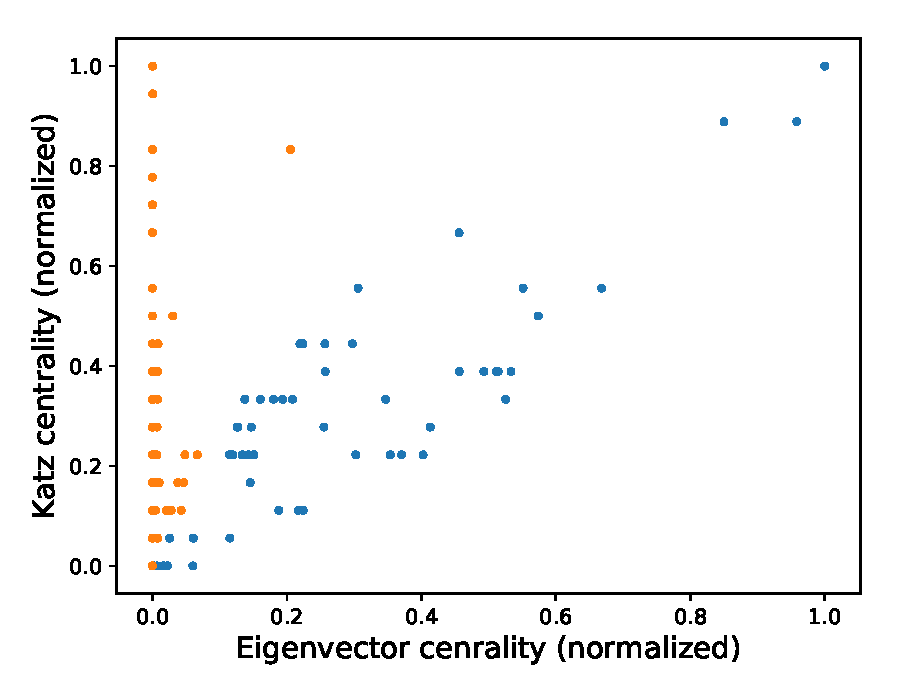
\includegraphics[width=0.45\linewidth]{amzn_product_ke_plot.eps}}
	\end{figure}
\end{frame}

\begin{frame}{KE Plot Identifies Communities in Real-World Networks (cont.)}
	\begin{figure}
		\centering
		\subfigure[Amazon health network\cite{amazon}]{
			\label{fig:amazon_health}
			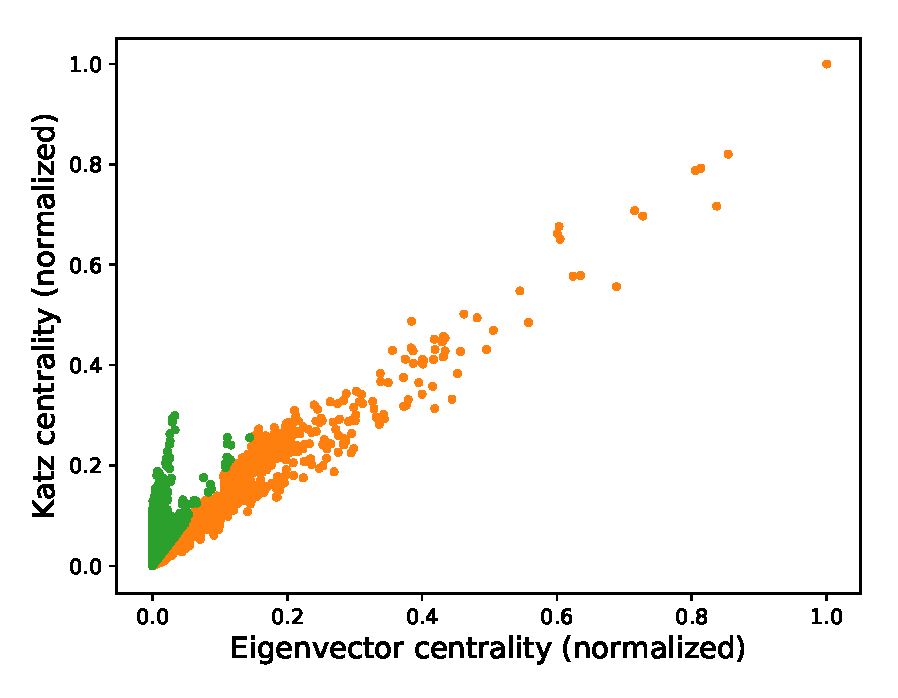
\includegraphics[width=0.45\linewidth]{amzn_health_ke_plot.eps}}
		\subfigure[Amazon beauty network\cite{amazon}]{
			\label{fig:amazon_beauty}
			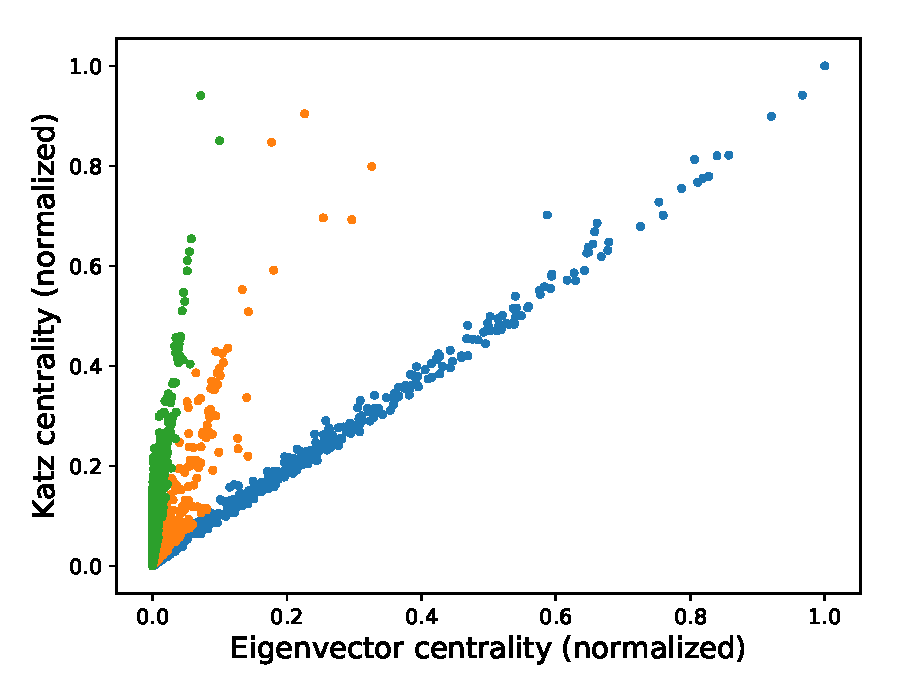
\includegraphics[width=0.45\linewidth]{amzn_beauty_ke_plot.eps}}
		\label{fig:all_examples}
	\end{figure}
\end{frame}

\begin{frame}{KE Method Performs Competitively Against Louvain and Spectral}
	\begin{table}
		\centering
		%\begin{tabular}{l@{\hskip 6mm}c@{\hskip 4mm}c@{\hskip 8mm}c@{\hskip 4mm}ccc}
		\begin{tabular}{lccc}
			\toprule
			& \multicolumn{3}{c}{\textbf{Runtime}} \\
			\midrule
			\textbf{Network} & \textbf{L} & \textbf{S} & \textbf{KE} \\
			\midrule
			AMZN Product& 371 ms  & 231 ms & 32 ms  \\
			AdHoc BA 1  & 11.8 s  & 877 ms & 329 ms \\
			AdHoc BA 2  & 2.03 m  & 3.88 s & 228 ms \\
			DBLP        & 12.0 m  & 1.15 hr& 751 ms \\
			AdHoc BA 3  & 2.07 hr & 4.65 m & 1.97 s \\
			AMZN Beauty & 11.7 hr & 14.5 m & 11.8 s \\
			AMZN Health & 16.2 d  & 5.30 m & 35.7 s \\
			\bottomrule
		\end{tabular}
		\caption{Comparison of runtime between Louvain community detection (\textbf{L}), spectral community detection (\textbf{S}), and the KE plot method of extracting communities from various networks with $n$ nodes and $m$ edges.}
		\label{tab:quality}
	\end{table}
\end{frame}

\begin{frame}{KE Method Performs Competitively Against Louvain and Spectral}
	\begin{table}
		\centering
		%\begin{tabular}{l@{\hskip 6mm}c@{\hskip 4mm}c@{\hskip 8mm}c@{\hskip 4mm}ccc}
		\begin{tabular}{lccc}
			\toprule
			& \multicolumn{3}{c}{\textbf{Modularity ($Q/Q_{max}$)}}\\
			\midrule
			\textbf{Network} & \textbf{L} & \textbf{S} & \textbf{KE}\\
			\midrule
			AMZN Product&  0.801/0.908 & 0.781/0.893 & 0.359/0.467 \\
			AdHoc BA 1  &  0.485/0.491 & 0.485/0.490 & 0.480/0.498 \\
			AdHoc BA 2  &  0.291/0.930 & 0.454/0.464 & 0.228/0.471 \\
			DBLP        &  0.805/0.982 & 0.713/0.974 & 0.019/0.034 \\
			AdHoc BA 3  & 0.203/0.931 & 0.382/0.393 & 0.123/0.492 \\
			AMZN Beauty & 0.499/0.840 & 0.566/0.735 & 0.365/0.645 \\
			AMZN Health & 0.413/0.543 & 0.00/0.00 & 0.423/0.608 \\
			\bottomrule
		\end{tabular}
		\caption{Comparison of resulting modularity between Louvain community detection (\textbf{L}), spectral community detection (\textbf{S}), and the KE plot method of extracting communities from various networks with $n$ nodes and $m$ edges.}
		\label{tab:quality}
	\end{table}
\end{frame}

\begin{frame}{KE Method Performs Competitively Against Louvain and Spectral}
	\begin{table}
		\centering
		%\begin{tabular}{l@{\hskip 6mm}c@{\hskip 4mm}c@{\hskip 8mm}c@{\hskip 4mm}ccc}
		\begin{tabular}{lccc}
			\toprule
			& \multicolumn{3}{c}{\textbf{Communities}}\\
			\midrule
			\textbf{Network} & \textbf{L} & \textbf{S} & \textbf{KE} \\
			\midrule
			AMZN Product&  14 & 17 & 3\\
			AdHoc BA 1  &  2 & 2 & 3\\
			AdHoc BA 2  &  17 & 2 & 2\\
			DBLP        &  129 & 191 & 2\\
			AdHoc BA 3  &  18 & 3 & 2\\
			AMZN Beauty &  25 & 4 & 3\\
			AMZN Health &  34 & 1 & 2\\
			\bottomrule
		\end{tabular}
		\caption{Comparison of the number of detected communities between Louvain community detection (\textbf{L}), spectral community detection (\textbf{S}), and the KE plot method of extracting communities from various networks with $n$ nodes and $m$ edges.}
		\label{tab:quality}
	\end{table}
\end{frame}

\begin{frame}{KE Method Supported By Louvain Results}
	\begin{figure}
			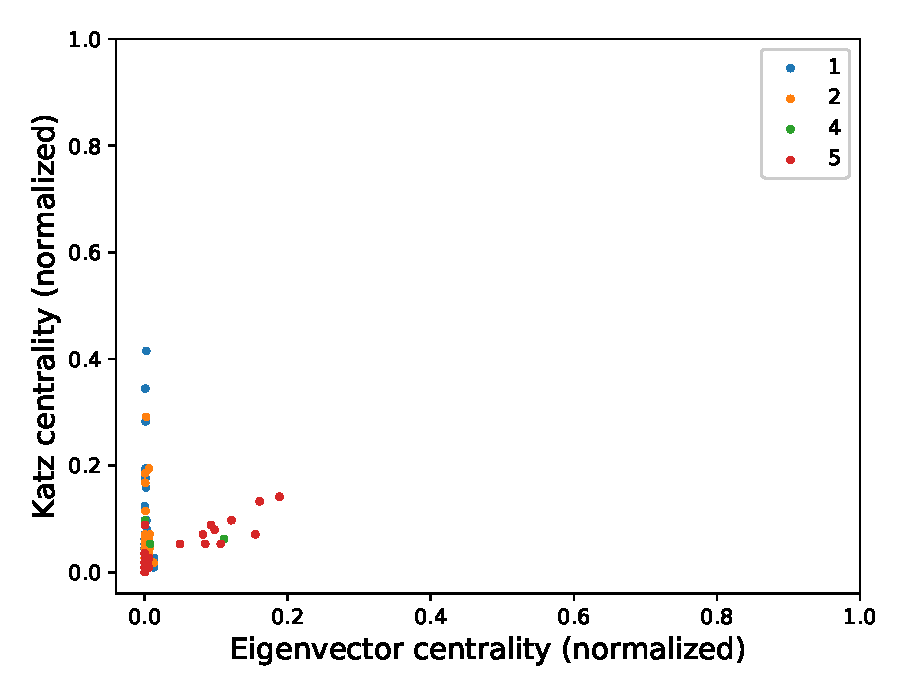
\includegraphics[width=0.5\textwidth]{louvain1.eps}%
			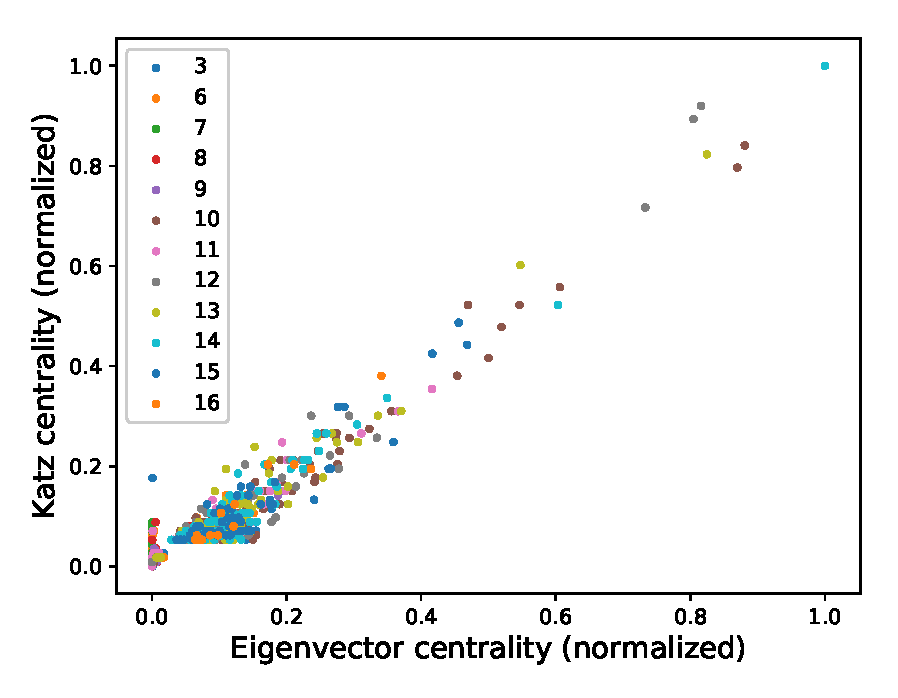
\includegraphics[width=0.5\textwidth]{louvain2.eps}
		\caption{16 communities within an ad-hoc modular network detected using Louvain, reduced to two groups that largely follow the pattern utilized by the KE method.}
		\label{fig:louv}
	\end{figure}
\end{frame}

\begin{frame}{Thank You}
	\centering
	Supporting code available at \href{https://github.com/markditsworth/modularity_study}{github.com/markditsworth/ModularityStudy}
\end{frame}

\begin{frame}{Appendix A: Clustering Algorithm}
	\begin{figure}
		\centering
		\subfigure[]{
			\label{fig:scatter}
			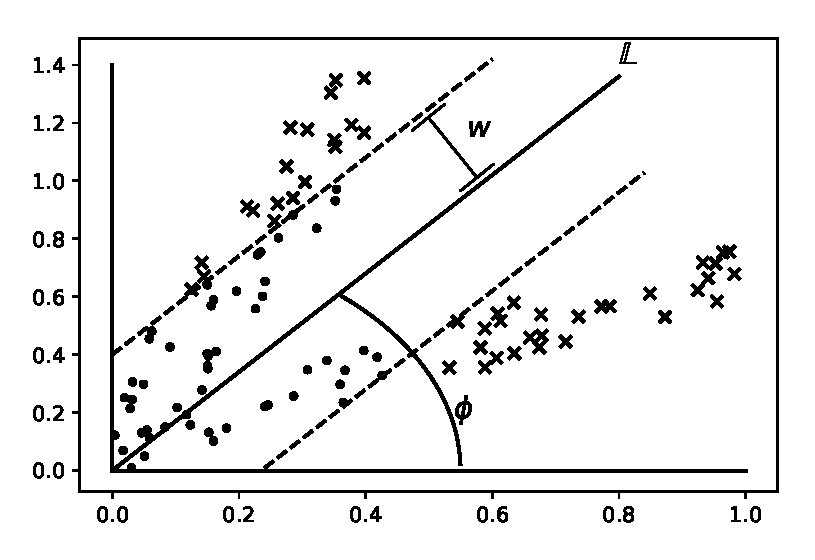
\includegraphics[width=0.48\linewidth]{scatter.eps}}
		\subfigure[]{
			\label{fig:curve}
			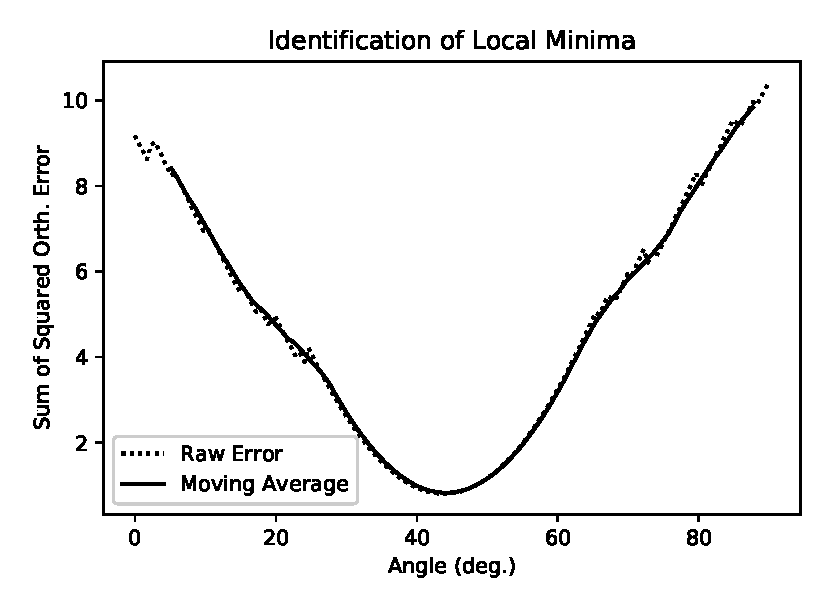
\includegraphics[trim={0 0 0 0.65cm},clip,width=0.48\linewidth]{curve.eps}}
		\label{fig:clustering}
	\end{figure}
\end{frame}

\begin{frame}{Appendix B: KE Plot Example using Erdos-Renyi model}
	
	\begin{figure}
		\centering
		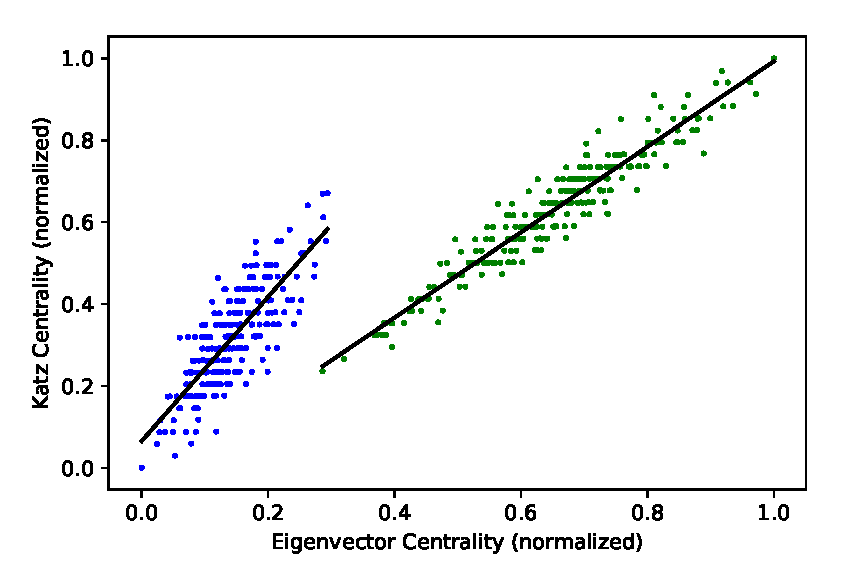
\includegraphics[scale=0.6]{./example_er}
		\caption{Ad-hoc modular network with two Erdos-Renyi\cite{er} random networks (n=250) joined by 800 randomly placed edges.}
	\end{figure}
\end{frame}

\begin{frame}{Appendix C: Modularity, Density Affect The KE Plot Clusters' Angle (ER)}
	\begin{figure}
		\centering
		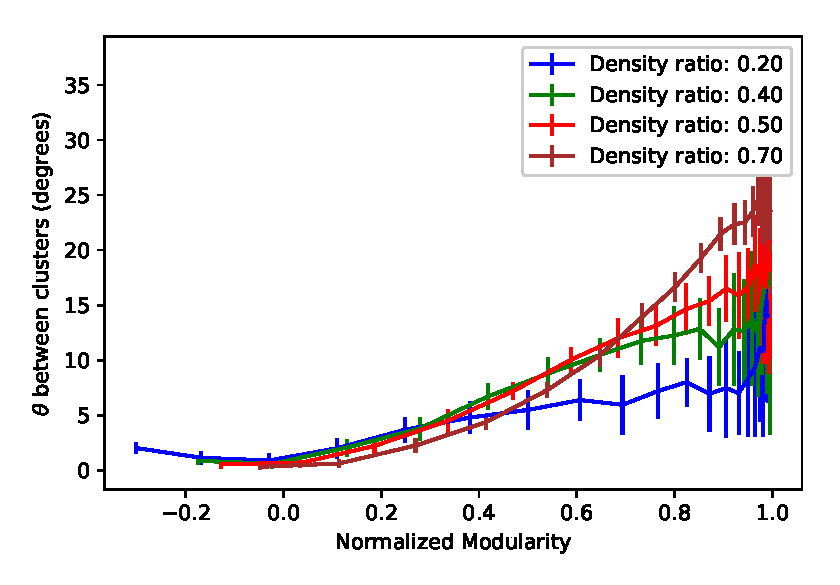
\includegraphics[scale=0.7]{theta_er.eps}
	\end{figure}
\end{frame}

\begin{frame}{Appendix D: Modularity, Density Affect The KE Plot Clusters' Distance (ER)}
	\begin{figure}
		\centering
		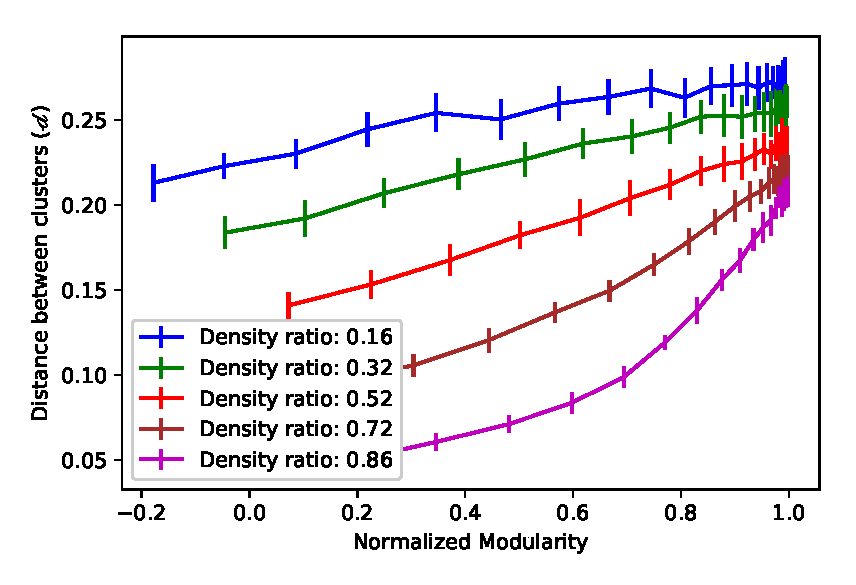
\includegraphics[scale=0.7]{distance_ba.eps}
	\end{figure}
\end{frame}

\begin{frame}{Appendix E: Modularity, Density Affect The KE Plot Clusters' Length Ratio (ER)}
	\begin{figure}
		\centering
		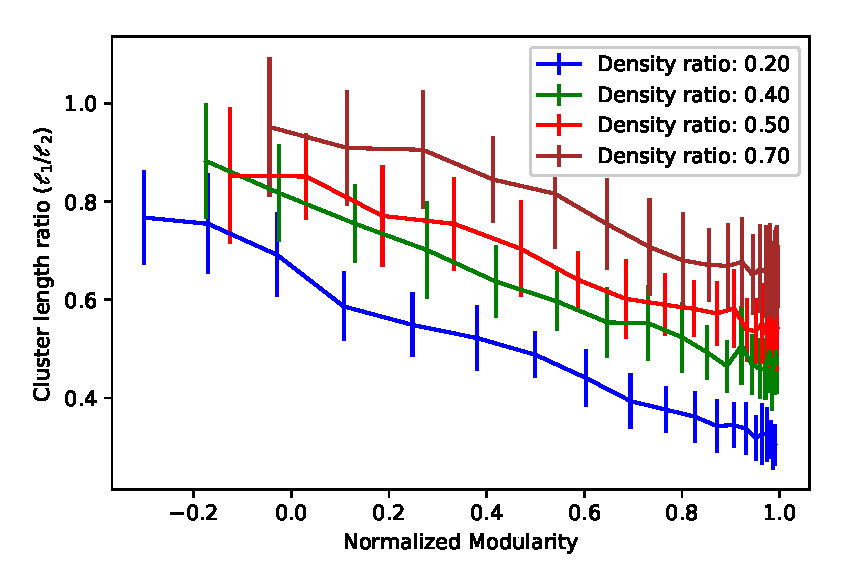
\includegraphics[scale=0.7]{length_er.eps}
	\end{figure}
\end{frame}

\begin{frame}[allowframebreaks]{References}
	\bibliographystyle{amsalpha}
	\bibliography{refs}
\end{frame}
\end{document}
